%---------------------------------------------------------
%	APPENDIX (backup slides, not counted)
%---------------------------------------------------------
\appendix

\begin{frame}[noframenumbering]
    \frametitle{Backup: Dataset Scale}
    \framesubtitle{Paired datasets, number of image pairs (README)}

    \begin{center}
        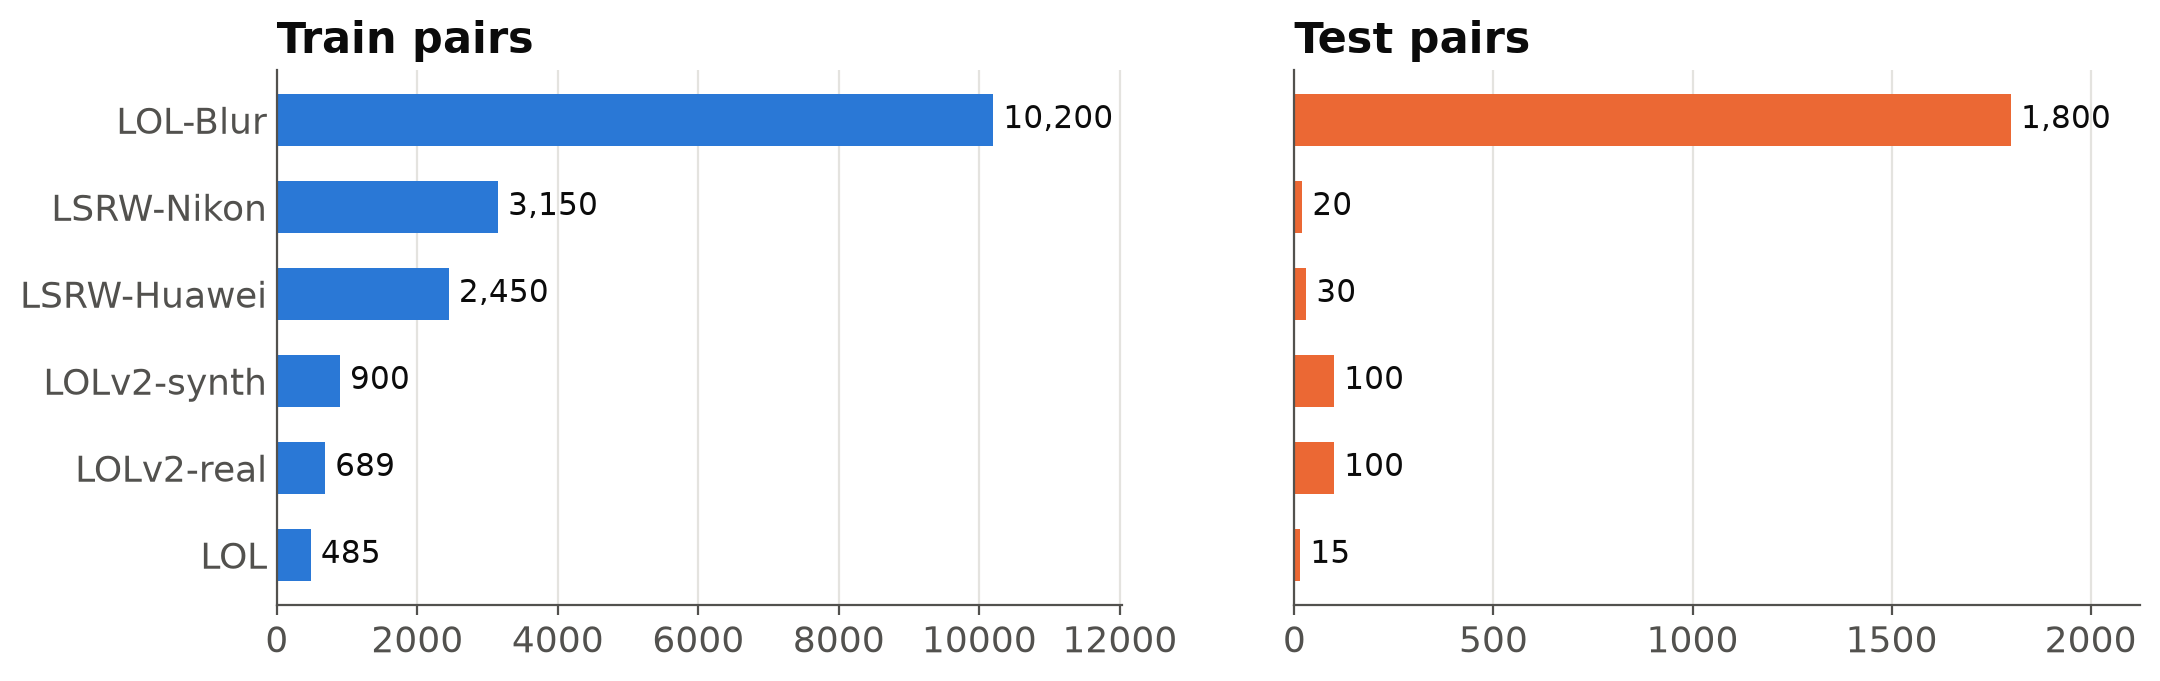
\includegraphics[width=0.95\textwidth]{eda/dataset_sizes.png}
    \end{center}
    {\footnotesize
    \begin{itemize}
        \item LOL-Blur alone has more training pairs than all other paired sets combined.
        \item Test sets are tiny for LOL (15) and LSRW (20--30): single-number scores there are noisy.
    \end{itemize}
    }
\end{frame}

\begin{frame}[noframenumbering]
    \frametitle{Backup: LOLv2 Samples}
    \framesubtitle{Low-light input (top) vs.\ normal-light ground truth (bottom), test split}

    \begin{center}
        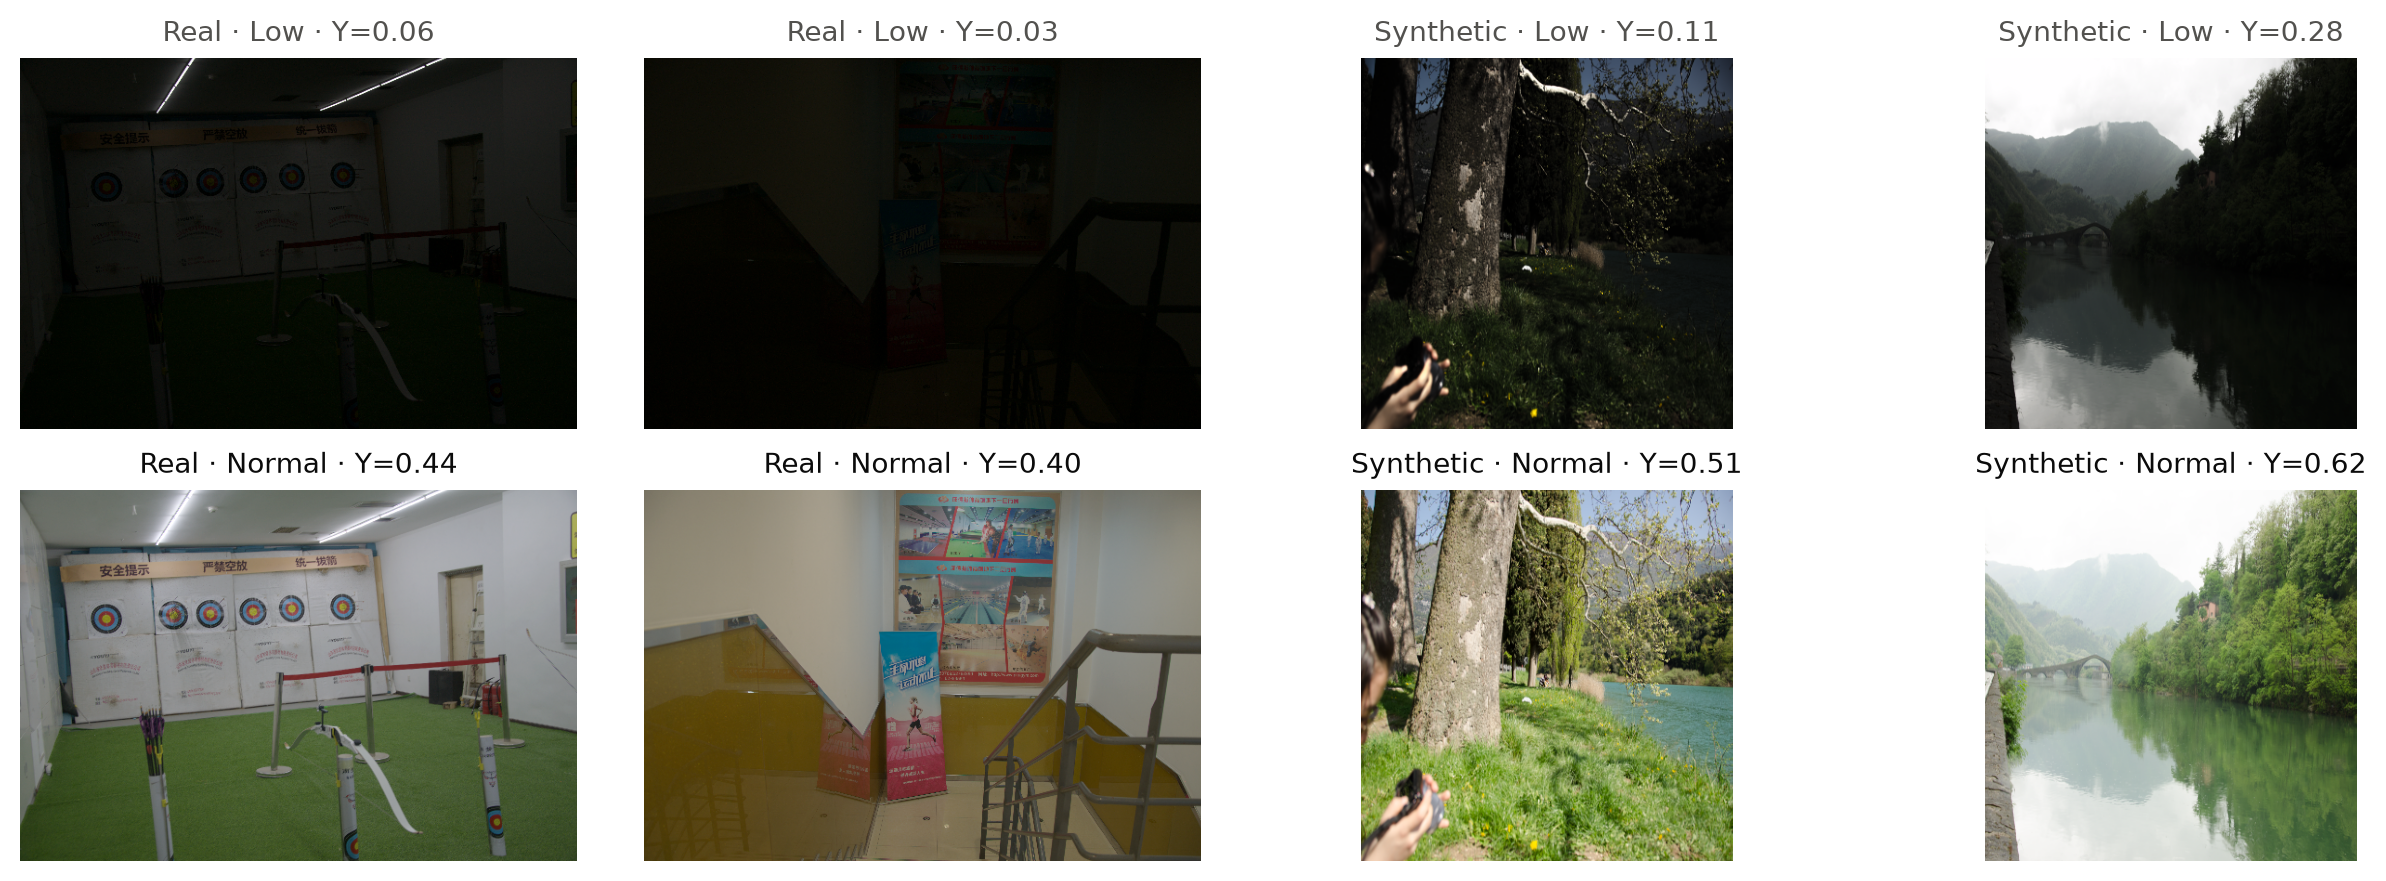
\includegraphics[width=\textwidth, height=0.6\textheight, keepaspectratio]{eda/samples.png}
    \end{center}
    {\footnotesize
    \begin{itemize}
        \item Real: 689 + 100 pairs, 600$\times$400. Synthetic: 900 + 100 pairs, 384$\times$384. All RGB, every low image has its ground truth.
    \end{itemize}
    }
\end{frame}
